\documentclass{ctexart}

\usepackage{lipsum}
\usepackage{hyperref}
\usepackage[margin=1in,left=1.5in,includefoot]{geometry}
\usepackage{listings}
\usepackage{xcolor}
\usepackage{amsmath}
\usepackage{geometry}
\usepackage{amsmath}
\usepackage{graphicx}
\usepackage{subfigure}
\usepackage{float}
\lstset{
    basicstyle=\footnotesize,
    %行号
    numbers=left,
	 breaklines=true,   
    rulesepcolor=\color{red!20!green!20!blue!20},
    escapeinside=``,
    xleftmargin=2em,
	 xrightmargin=2em, 
	 %aboveskip=1em,
    %背景框
    %framexleftmargin=1.5mm,
    frame=shadowbox,
	 %breakatwhitespace=false,
	 flexiblecolumns=true,
    %背景色
    backgroundcolor=\color[RGB]{245,245,245},
    %样式
    keywordstyle=\color{blue}\bfseries,
    identifierstyle=\bf,
    numberstyle=\color[RGB]{0,192,192},
    commentstyle=\it\color[RGB]{96,96,96},
    stringstyle=\rmfamily\slshape\color[RGB]{128,0,0},
    %显示空格
    showstringspaces=false,
	 escapechar=`
 }

% \geometry{screen}
%\lstset{
    %numbers=left, 
    %numberstyle= \tiny, 
    %keywordstyle= \color{ blue!70  },
    %commentstyle= \color{red!50!green!50!blue!50}, 
    %frame=shadowbox, % 阴影效果
    %rulesepcolor= \color{ red!20!green!20!blue!20  },
    %escapeinside=`, % 英文分号中可写入中文
    %xleftmargin=2em,xrightmargin=2em, aboveskip=1em,
    %framexleftmargin=2em
%} 
% Heading and Footer Stuff
\usepackage{fancyhdr}
\hypersetup{
    colorlinks=true,
    bookmarks=true,
    %bookmarksopen=false,
    % pdfpagemode=FullScreen,
    % pdfstartview=Fit,
    pdftitle={算法分析与报告},
    pdfauthor={周翔辉}
}
\pagestyle{fancy}
\fancyhead{}
\fancyfoot{}
% For right foot page number
\fancyfoot[R]{第{\thepage}页}
\renewcommand{\headrulewidth}{0pt}
% 页面下方的线
\renewcommand{\footrulewidth}{0.5pt}

\newcommand\tab[1][1cm]{\hspace*{#1}}

\begin{document}

\begin{titlepage}
    \begin{center}
        \line(1,0){0} \\
        [0.25in]
        \huge{\bfseries 《算法分析与设计》} \\
        [0.25in]
        \huge{\bfseries 课程设计报告} \\
        \line(1,0){0} \\
        [2mm]
        \line(1,0){0} \\
        [5cm]
        {
            \zihao{-2}
        \begin{tabular}{cc}
            学院(系): & 软件工程系 \\
            班级: & 116030801 \\
            学生姓名: &  周翔辉\\
            学号: & 11603080122 \\
            指导老师: &刘祥 \\
            [2cm]
        \end{tabular}

        {\bfseries 时间: 从2018年12月17日到2018年12月27日}\\
        }
    \end{center}
\end{titlepage}

\pagenumbering{roman}
\tableofcontents
\cleardoublepage

\newpage
\pagenumbering{arabic}

\setcounter{page}{1}

\section{基本的递归算法}
\subsection{二项式的计算}
\subsubsection{问题描述}
完成二项式公式计算,即 $C_n^k = C_{n-1}^{k-1} + C_{n-1}^k$ 公式解释为了从 $n$ 个不同元素
中抓取 $k$ 个元素 ($C_n^k$),可以这样考虑,如果第一个元素一定在结果中,那么就需要从剩下的 $n-1$ 个
元素中抓取 $k-1$ 个元素 ($C_{n-1}^{k-1}$);如果第一个元素不在结果中,就需要从剩下的 $n-1$ 个元素中抓取 $k$个元素
($C_{n-1}^k$)。要求分别采用以下方法计算,并进行三种方法所需时间的经验分析。
\subsubsection{解决问题所用的算法设计方法及基本思路}
此问题可以通过下面的算法实现:
\begin{enumerate}
    \item {\bfseries 递归算法}
    考虑计算 $C_n^k$ 的情况, $C_n^k = C_{n-1}^{k-1} + C_{n-1}^k$, 则可以递归的调用此方法或者函数,\\
    直到 $n$ 和 $k$ 有一个为 $1$ 就返回 $1$, $k=1$ 时就返回 $n$ 。
    \item {\bfseries 备忘录方法} 需要借助上面的 {\bfseries 递归算法}, 当 $C_{n-i}^{k-j}$ 不等于 $0$ 时,
    就计算这个值,然后保存到一个数组中,其它公式如果需要它的值则直接从数组中调用即可,不需要再次计算。
    \item {\bfseries 迭代算法} 通过一个结果二维数组保存从 $C_1^1$ 到 $C_n^k$ 的所有值,从小到大计算,逐行填表。\\
\end{enumerate}
\subsubsection{采用的数据结构描述}
在{\bfseries 递归算法}中,系统底层采用栈存储递归的数据,然后逐层返回;在{\bfseries 备忘录方法}中采用了一个额外的二维
数组来保存中间过程的值;在{\bfseries 迭代算法}中,也是通过一个二维数组实现逐行填表,计算二项式公式的值。
\subsubsection{算法描述}
\begin{enumerate}
    \item {\bfseries 递归算法} \\
	{\bfseries{算法 CalculateBinomialRecursion $(k, n)$ }} \\
	\tab// 计算二项式公式 使用递归 \\
	\tab// 输入:二项式公式的 $k, n$ \\
	\tab// 输出:二项式公式的值 \\
	\tab{\bfseries{if}} $k > 0$ \&\& $n > 0$ \\
	\tab\tab{\bfseries{if}} $k = 1$ and $n = 1$ \\
	\tab\tab\tab{\bfseries{return}} 1 \\
	\tab\tab{\bfseries{else if}} $k = 1$ \\
	\tab\tab\tab{\bfseries{return}} n \\
	\tab\tab{\bfseries{else}} \\
	\tab\tab\tab{\bfseries{return}} CalculateBinomialRecursion $(k-1,n-1)$ \\
	\tab\tab\tab+ CalculateBinomialRecursion $(k,n-1)$\\
	\tab{\bfseries{return}} 0

   \item {\bfseries 备忘录算法} \\
	{\bfseries{算法 CalculateBinomialMemo $(k, n)$ }} \\
	\tab// 计算二项式公式 使用备忘录方法 \\
	\tab// 输入:二项式公式的 $k, n$ \\
	\tab// 输出:二项式公式的值 \\
	\tab// 注意:$C[n,k]$ 用于保存中间过程的值,减少重复计算\\
	\tab{\bfseries{if}} $k > 0$ \&\& $n > 0$ \\
	\tab\tab{\bfseries{if}} $k = 1$ and $n = 1$ \\
	\tab\tab\tab{\bfseries{return}} 1 \\
	\tab\tab{\bfseries{else if}} $k = 1$ \\
	\tab\tab\tab{\bfseries{return}} n \\
	\tab\tab{\bfseries{else}} \\
	\tab\tab\tab$c[k,n]=$ CalculateBinomialRecursion $(k-1,n-1)$ \\
	\tab\tab\tab+ CalculateBinomialRecursion $(k,n-1)$\\
	\tab{\bfseries{return}} $c[k,n]$ \\
	{\bfseries return} 0

   \item {\bfseries 迭代算法} \\
	{\bfseries{算法 CalculateBinomialIteration $(k, n)$ }} \\
	\tab// 计算二项式公式 使用迭代方法 \\
	\tab// 输入:二项式公式的 $k, n$ \\
	\tab// 输出:二项式公式的值 \\
	kns $\leftarrow$ array\
	{\bfseries for} $i = 0$ to n \\
	\tab {\bfseries for } $j = 0$ to $k$ \\
	\tab {\bfseries if} $i < j$ \\
	\tab\tab $kns[i][j] = 0$ \\
	\tab {\bfseries else if} $j == 1$ \\
	\tab\tab $kns[i][j] = i$ \\
	\tab {\bfseries else if} $j == j$ \\
	\tab\tab $kns[i][j] = 1$ \\
	\tab {\bfseries else} \\
	\tab\tab $kns[i][j] = kns[i-1][j-2] + kns[i-1][j-1]$ \\
	{\bfseries return} kns[n-1][k-1]
\end{enumerate}
\subsubsection{算法的时间空间复杂度分析}
下面是几种算法的运行时间的时间和 $k$ 曲线图
\begin{figure}[H]
	\centering
	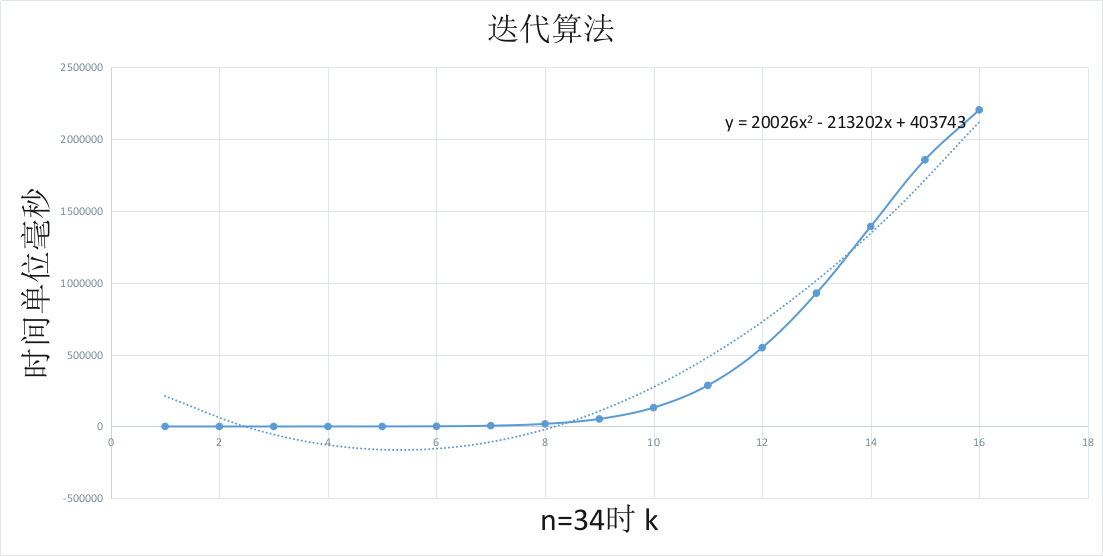
\includegraphics[scale=0.5]{../images/recursion.png}
	\caption{递归算法}
\end{figure}

\begin{figure}[H]
	\centering
	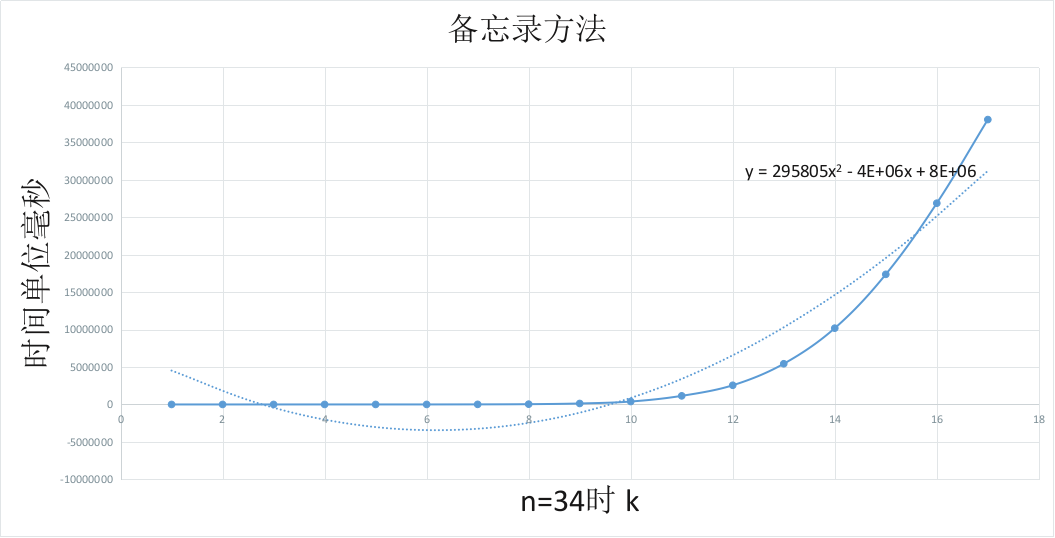
\includegraphics[scale=0.5]{../images/memo.png}
	\caption{备忘录方法}
\end{figure}

\begin{figure}[H]
	\centering
	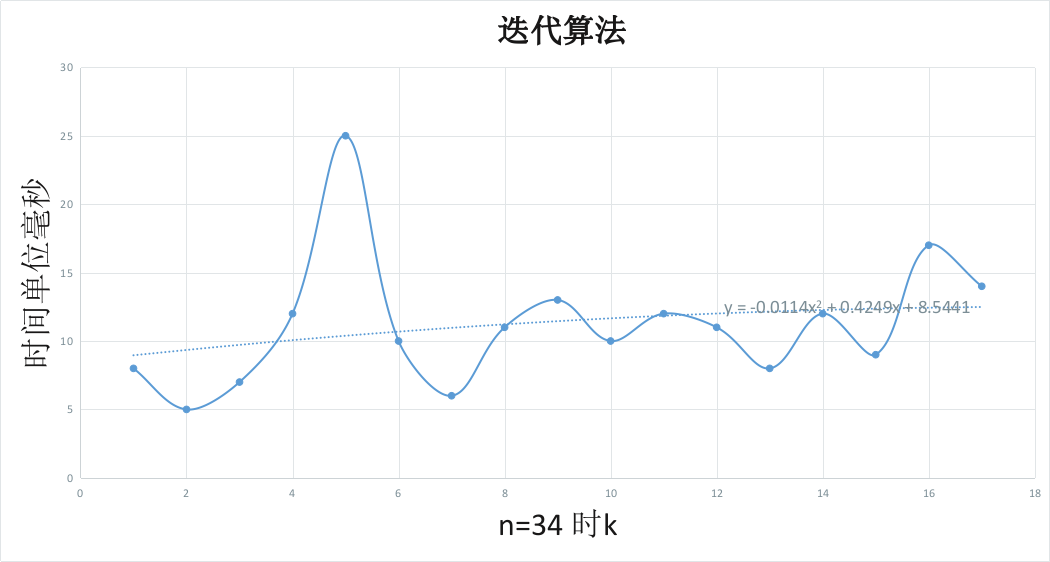
\includegraphics[scale=0.4]{../images/iteration.png}
	\caption{迭代算法}
\end{figure}

通过分析,可以得出{\bfseries 递归算法}的时间复杂度 $\Theta(n) = n^2$,空间复杂
度为 $O(1)$ ;{\bfseries 备忘录方法}的时间复杂度 $\Theta(n) = n^2,
$空间复杂度为 $O(n)$ ;{\bfseries 迭代算法}的时间复杂度 $\Theta(n) = n^2$,
空间复杂度为 $O(n^2)$ 。
\subsubsection{算法实例}
输入:
\begin{lstlisting}[language=C]
n=16
k=7
\end{lstlisting}

输出:

\begin{figure}[H]
	\centering
	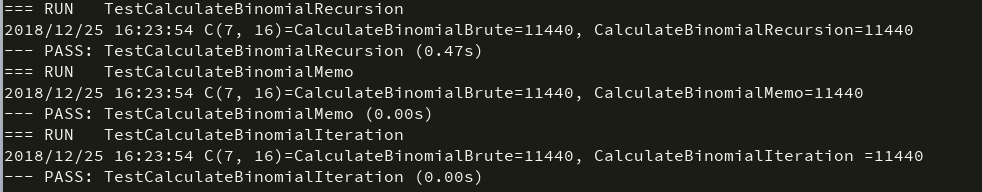
\includegraphics[scale=0.5]{../images/binomial-test.png}
	\caption{测试计算二项式的算法}
\end{figure}

\newpage
\subsection{绘制简单的分形树}
\subsubsection{问题描述}
\begin{figure}[H]
	\centering
	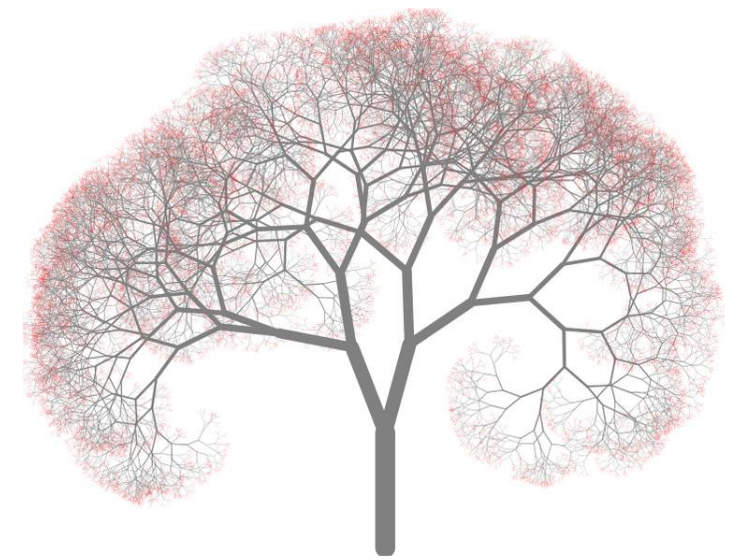
\includegraphics[scale=0.5]{../images/demo-tree.png}
	\caption{分形树示例}
\end{figure}

先垂直绘制一根线段,然后在线段顶端向右一定倾角绘制一根线段,长度分别为原线段的k倍. 再同样
的,在线段左侧以固定倾角绘制一根线段,如此反复,直至线段长度小于某个较小的值。其中,线条
颜色以及长度,夹角(例如产生某个范围的随机数)都可以自行进行微调。

\subsubsection{解决问题所用的算法设计方法及基本思想}
使用递归的思想,假定现在正在一个节点,那么随机生成两个角度和长度,调用画图的方法画出两个子节点,
然后再递归的画出这两个子节点的图。
\subsubsection{采用的数据结构描述}
无。
\subsubsection{算法描述 }
   {\bfseries 绘制简单的分形树算法} \\
	\tab{\bfseries{算法 ddraw $(x, y, length, angle)$ }} \\
	\tab// 绘制简单的分形树 递归算法 \\
	\tab// 输入:节点的$x, y$ 表示坐标, $length$ 表示长度, $angle$ 表示偏的角度 \\
	\tab// 输出:绘制出的分形树的图像 \\
	\tab{\bfseries if} $length < minilength $// 最短的边长度,退出条件 \\
	\tab\tab{\bfseries return} \\
	\tab $x_2,y_2,x_3,y_3 = $ getRandomSon(x,y) // 获取子节点的坐标 \\
	\tab draw($x,y,length,angle$)// 画出当前节点 \\
	\tab ddraw($x_2,y_2,randomLength_2,randomAngle_2$) // 画左边子节点 \\
	\tab ddraw($x_3,y_3,randomLength_3,randomAngle_3$) // 画右边子节点 \\

\subsubsection{算法的时间空间复杂度分析 }
假定树的深度为 $n$ ,那么此算法的时间复杂度为 $\Theta(n) = 2^n$,空间复杂度也为 $2^n$ 。 
\subsubsection{算法实例}
下面是一个随机生成的分形树的实例:
\begin{figure}[H]
	\centering
	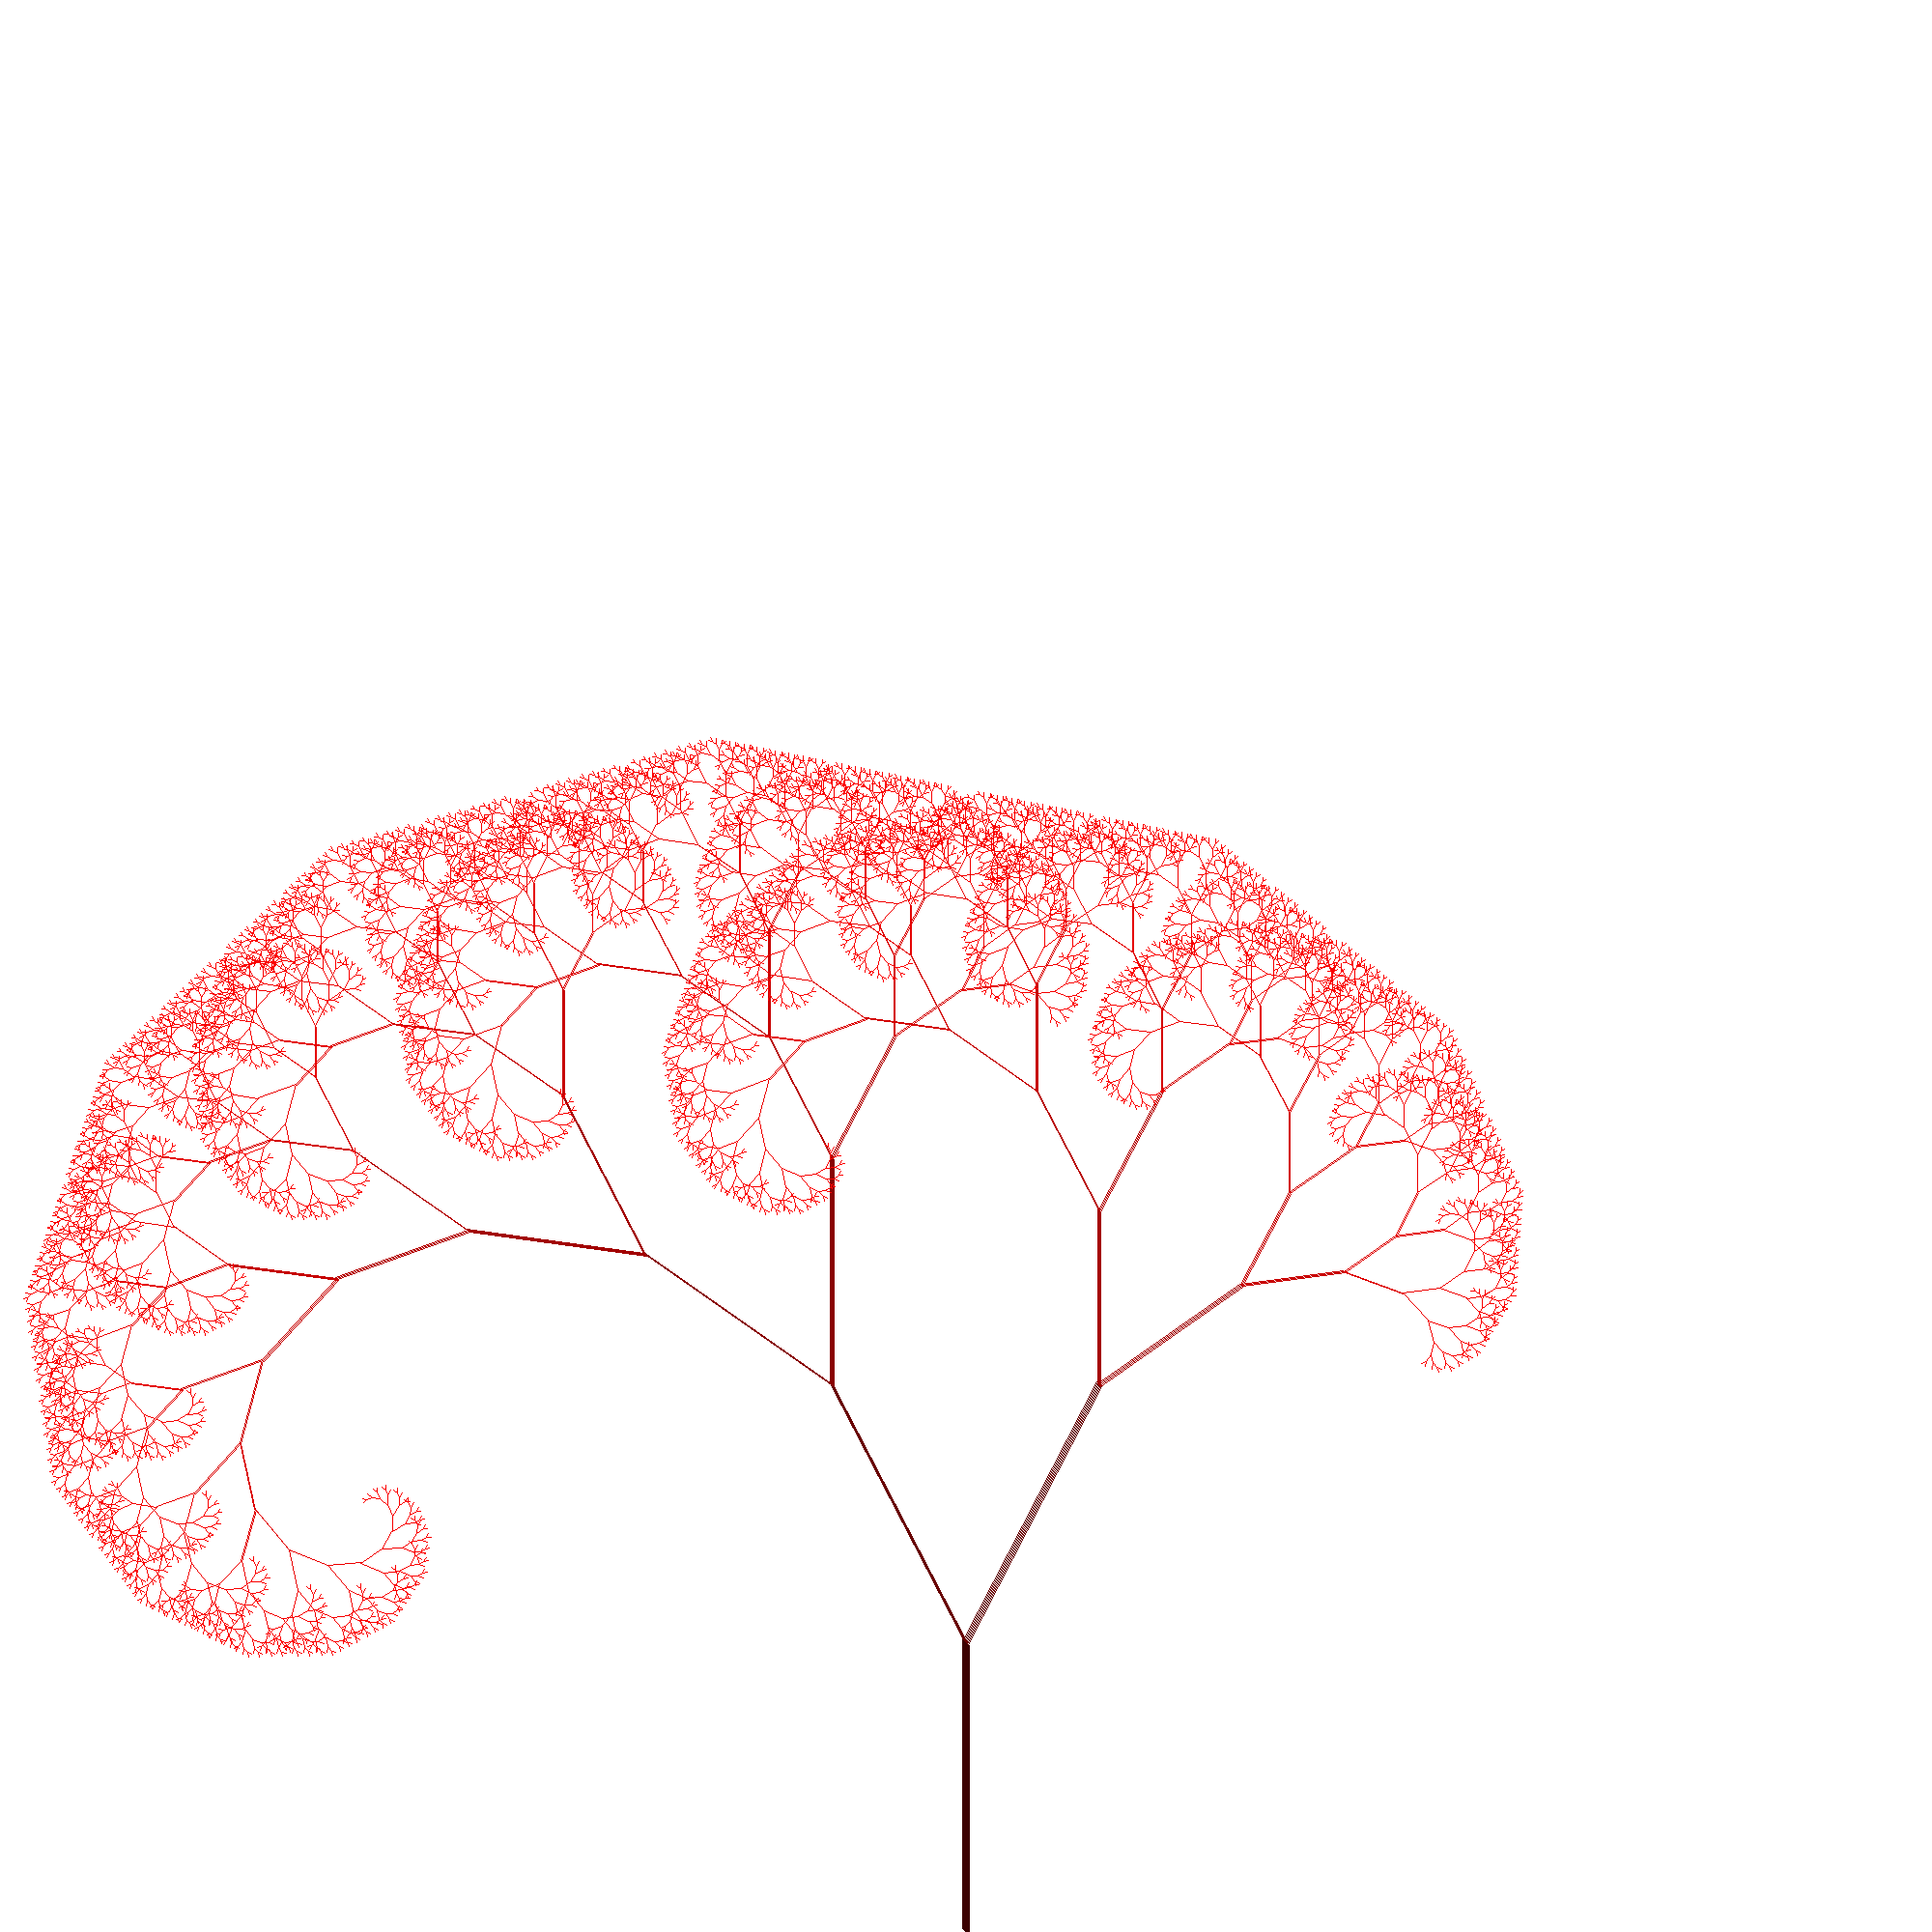
\includegraphics[scale=0.15]{../images/trree.png}
	\caption{生成的分形树的实例}
\end{figure}

\newpage
\section{遍历}
\subsection{8品脱问题}
\subsubsection{问题描述}
西蒙.丹尼斯.泊松是著名的法国数学家和物理学家。据说在他遇到某个古老的谜题之后,就开始对数学
感兴趣了,这个谜题是这样的:给定一个装满水的8品脱壶以及两个容量分别为5品脱和3品脱的空
壶,如何通过完全灌满或者到空这些壶从而使得某个壶精确地装有4品脱的水?用广度优先查找来求解
这个谜题。要求在输出结果中包含广度优先的遍历过程(结点的遍历顺序)。
\subsubsection{解决问题所用的算法设计方法及基本思想}
采用广度有序一层一层遍历的思想,考虑某一层中的某个节点(这棵树中每个节点都保存着当前每个瓶子的信息,包括
容量和已经使用了多少),这几个瓶子可以互相倒水,只有能够倒成功的才能进行下一步,并且倒水后的节点不能已经
存在,这样一层一层的倒水,当某个节点满足添加时即可退出,并倒序回去得到倒水过程。
\subsubsection{采用的数据结构描述}
使用了一个栈来保存树的节点,一个数组来保存已经产生的结果(用来判断这个节点是否已经产生过了),一个结构体
来保存瓶子的容量和用量。
\subsubsection{算法描述 }
   {\bfseries 找到一个倒水过程使其符合给定的结果} \\
   \tab{\bfseries{算法 find $(nodes)$ }} \\
	\tab// 找到一个倒水过程使其符合给定的结果\\
	\tab// 输入:一个或多个起始状态节点数组 nodes \\
	\tab// 输出:到给定结果的倒水过程\\
	\tab{\bfseries if} $len(nodes) \leftarrow 0$ \\
	\tab\tab{\bfseries return} null \\
	\tab cloneNode $\leftarrow$ clone(nodes) // 复制当前所有节点信息 \\
	\tab newNodes $\leftarrow$ array // 创建一个新的数组保存生成的所有节点 \\
	\tab{\bfseries for} node in cloneNode {\bfseries do} // 遍历这层的所有节点 \\
	\tab\tab{\bfseries for} bottle1 in node // 每个节点的瓶子互相倒水 \\
	\tab\tab{\bfseries for} bottle2 in node // 每个节点的瓶子互相倒水 \\
	\tab\tab\tab{\bfseries if} $bottle1 \ne bottle2$ {\bfseries do} // 瓶子不同才倒水\\
	\tab\tab\tab// 先克隆,后倒水				\\
	\tab\tab\tab newNode=pour(bottle1,bottle2,node) \\
	\tab\tab\tab{\bfseries if} newNode isnot in nodeLists {\bfseries do} \\
	\tab\tab\tab\tab nodeList.add(newnode) // 全局保存的所有节点\\
	\tab\tab\tab\tab newNodes.add(newnode) \\
	\tab\tab\tab\tab newNode.parent = node // 使当前节点的父节点志向node\\
	\tab\tab\tab{\bfseries if} Has(newNode, number) // 判断当前节点是否满足退出条件 \\
	\tab\tab\tab\tab{\bfseries return} newNode \\
	\tab find(newNodes)
\subsubsection{算法的时间空间复杂度分析 }
时间复杂度 $\Theta(n) = n^2$ ,空间辅助度为 $n^2$
\subsubsection{算法实例}

输入:
\begin{lstlisting}[language=C]
// 瓶子数组 容量、用量
[{122,99}, {50,25}, {12,1}, {2,0}, {5,4}] 
40 // 需要的结果
\end{lstlisting}

输出:
\begin{figure}[H]
	\centering
	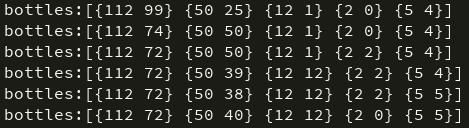
\includegraphics[scale=0.6]{../images/eight_pints_result_demo.png}
	\caption{品脱倒水问题结果}
\end{figure}

\newpage
\subsection{24点问题}
\subsubsection{问题描述}
用户输入4位个位数(1~9),四个数之间只能通过+,-,*,/运算进行连接,请输出四则运算表达式,其
求值结果为24。然后输出所有求值结果为24的组合。你能不能不通过四重循环来产生这4个参与运算
的数。
\subsubsection{解决问题所用的算法设计方法及基本思想}
可以使用如下的不在求解:
\begin{enumerate}
	\item 产生4个数的排列;
	\item 产生运算符的排列(4种运算符,任选3个);
	\item 考虑加括号方式,纸上推演一下,有5种加括号方式,如果对4个数的排列没有约束,加括号方式
也可以简化为三种< $(a+b)+(c+d), ((a+b)+c)+d, (a+(b+c))+d>。a+((b+c)+d),a+(b+(c+d))$ 是被去掉的两种,这里加号表示运算符。
\end{enumerate}

然后循环数的排列、运算符的排列和三个加括号的方式,一一计算,即可以求出哪些可以满足24点。
\subsubsection{采用的数据结构描述}
使用数组来保存生成的数的排列和运算符的排列,使用字符串数组来保存满足24点的表达式。
\subsubsection{算法描述 }
   {\bfseries 计算24点} \\
	\tab{\bfseries{算法 CalculatePoints$($a, b, c, d$)$ }} \\
	\tab// 计算24点 \\
	\tab// 输入:$a,b,c,d$ 四个个位数 \\
	\tab// 输出:所有满足24点的表达式 \\
	\tab resultList $\leftarrow$ array // 保存符号24点的表达式数组 \\
	\tab expressionList $\leftarrow $getPerms($a,b,c,d$) // 获取 $a,b,c,d$ 构成的排列 \\
	\tab operatorList $\leftarrow$ getOperator("+","-","*","/") // 获取 $+,-,*,/$ 构成的排列 \\
	\tab{\bfseries for} $i \leftarrow 0$ to len(expressionList) {\bfseries do}\\
	\tab\tab{\bfseries for} $j \leftarrow 0$ to len(expressionList) {\bfseries do}\\
	\tab\tab\tab if calculate(expressionList[i], operatorList[j]) $= 24$ //$(a+b) + (c+d)$ \\
	\tab\tab\tab resultList.add(expressionList[i]) \\
	\tab\tab\tab if calculate(expressionList[i], operatorList[j]) $= 24$ // $((a+b)+c)+d$ \\
	\tab\tab\tab resultList.add(expressionList[i]) \\
	\tab\tab\tab if calculate(expressionList[i], operatorList[j]) $= 24$ //$(a +(b+c)) + d$ \\
	\tab\tab\tab resultList.add(expressionList[i]) \\
	\tab{\bfseries return} resultList
\subsubsection{算法的时间空间复杂度分析 }
输入有4个数字,可以产生64种组合,4和运算符可以参数64种组合,还有3种情况,所以当输入梳子个数为 $n$ 时,则有 $n! * C_n^{n-1}*(n-1)! * c = cn!^2$, 
所以时间复杂度 $\Theta(n) = cn!^2$, 空间复杂度为 $cn!^2+k$ 。
\subsubsection{算法实例}
输入:
\begin{lstlisting}[language=C]
4,5,6,7 24
\end{lstlisting}

输出:
\begin{lstlisting}[language=C]
(4+(4/5))*6 (4-(4/5))*6 (4+(4/7))*6 (4-(4/7))*6 (6+6)*(7-5) 
(6*6)-(7+5) (6*6)-(5+7) (6/(6-5))*4 ((6/6)+5)*4 (6+(6/7))*4 
(6-(6/7))*4 (7-(7/5))*4 ((7/7)+5)*4 (7-7)+(4*6) ((7-7)+4)*6 
(7-7)+(6*4) ((7-7)+6)*4 (7-(7/6))*4 (7*7)/(6-4) (5*5)-(7/4) 
(5-5)+(6*4) ((5-5)+6)*4 (5*5)-(6/4) (5-5)+(4*6) ((5-5)+4)*6 
(5-(5/4))*6 ((5*5)-7)+6 (5*5)-(7/6) (5*5)+(6-7) ((5*5)+6)-7
\end{lstlisting}

\newpage
\section{动态规划}
\subsection{最长回文子序列问题}
\subsubsection{问题描述}
如果一个子序列从左向右和从右向左读都一样,则称之为回文。例如,序列 $ACGTGTCAAAATCG$ 有
很多回文子序列,比如 $ACGCA$ 和 $AAAA$ 。请给出一个算法,求出最长的回文子序列。
\subsubsection{解决问题所用的算法设计方法及基本思想}
将字符串中的每一个字符最开始时都当成一个回文子序列,然后遍历整个字符串,再遍历回文子序列的
数组,找到从字符 i 到这个字符的最大回文子序列,最后提取出最大的子序列。
\subsubsection{采用的数据结构描述}
使用一个 map 来保存子序列数组的下标, key 为 start,value 为 end。
\subsubsection{算法描述 }
   {\bfseries 找出最长的回文子序列} \\
	\tab{\bfseries{算法 find$(chars)$ }} \\
	\tab// 找出最长的回文子序列 \\
	\tab// 输入:$chars$ 需要寻找最长回文子序列的字符串\\
	\tab// 输出:$chars$ 中最长的回文子序列\\
	\tab result $\leftarrow$ array // 保存最长回文子序列的数组\\
	\tab resultMap $\leftarrow$ map // 保存最长回文子序列的start和end \\
	\tab // 初始化 最长回文子序列为字符串第一个元素 \\
	\tab{\bfseries for} $i \leftarrow 0$ to len(chars) {\bfseries do} \\
	\tab\tab resultMap[i] $\leftarrow $ = $i$ \\
	\tab{\bfseries for} $index \leftarrow 1$ to len(chars) {\bfseries do} \\
	\tab\tab{\bfseries for} $k,v $ range resultMap \\
	\tab\tab find($k,v,char,resultMap,index$) \\
	\tab// 找到resultMap中最长的元素value-key\\
	\tab longestLength $\leftarrow$ findLongestLength(resultMap) \\
	\tab// 找到chars中的最长回文子序列,长度为longestLength\\
	\tab result $\leftarrow$ findLongestSubString(longestLength,resultMap,chars) \\
	\tab{\bfseries return} result
\subsubsection{算法的时间空间复杂度分析 }
首先需要一个外层字符串的遍历,然后是寻找最长的回文子序列,其时间复杂度为
$\Theta(n) = n^3$,空间复杂度为 $n^2$。
\subsubsection{算法实例}
下面是实验测试过程中的一些输入输出:
\begin{figure}[H]
	\centering
	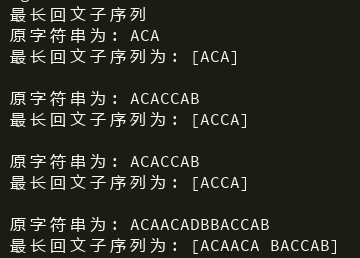
\includegraphics[scale=0.6]{../images/max_huiwen.png}
	\caption{最长回文子序列}
\end{figure}


\newpage
\subsection{小美购物问题}
\subsubsection{问题描述}
小美近来疯狂购物,信用卡上获得积分100000。在积分商城中有许多物品可以选兑。例如食用油,大
米,钢笔,电烤炉,研磨机,热水壶等等。信用卡积分就快过期了,小美想将这一万积分尽量用光,
请问小美应该怎么办?

小美在挑选物品的过程中,发现有些积分和实际价格的比例大概是100:1,继而发现有些商品在积分商
城里购买并不划算,不如去京东购买。小美为了这100000积分也是拼了,将所有商品在京东的价格罗
列了出来,同时罗列了所有商品的积分。此时小美又应该怎么挑选,使得获得的价值最大?(或许你
应该想想价值是什么?)
\subsubsection{解决问题所用的算法设计方法及基本思想}
此问题跟背包问题非常类似,都是价值最大化的问题,在一定的积分(重量)下,选择合适的商品(具有一定的积分和价值(重量和价值))
,使用一层一层的填表,即 $$F(i,j) = \Bigm\lbrace ^{F(i,j) = max{F(i-1,j), v_i + F(i-1,j-w_j), j-w_j \ge 0}} _{F(i-1,j), \tab j - w_j < 0}$$
\subsubsection{采用的数据结构描述}
使用一个二维数组保存填表的信息($F(i,j)$) 的值。
\subsubsection{算法描述 }
   {\bfseries 最大价值化问题} \\
   \tab{\bfseries{算法 FindMaxValue1(i,j,prices, credits, totalCredit) }} \\
	\tab// 找出价值最大的商品集合 \\
	\tab// 输入:prices 每个商品的价格\\
	\tab// 输入:credits 每个商品的积分\\
	\tab// 输入:totalCredit 一共拥有的积分\\
	\tab// 输出:最大价值商品的集合\\
	\tab// 注意:F数组除了行0和列0用0初始化外,其它全部用-1初始化\\
	\tab{\bfseries if} $F(i,j) < 0$  {\bfseries do} \\
	\tab\tab{\bfseries if} $j < credits[i]$ {\bfseries do} \\
	\tab\tab\tab $value \leftarrow FindMaxValue(i-1,j,prices,credits,totalCredit)$ \\
	\tab\tab{\bfseries else do} \\
	\tab\tab\tab $value \leftarrow max(FindMaxValue1(i-1,j)), \\
	prices[i] + FindMaxValue(i-1,j-credits[j-prices[i]])$\\
	\tab\tab $F[i,i] \leftarrow value$\\
	\tab{\bfseries return} $F[i,j] $
\subsubsection{算法的时间空间复杂度分析 }
此算法基于填表的查询相加,时间复杂度为 $\Theta(n) = (n+1)^2$,空间复杂度也为 $(n+1)^2$。
\subsubsection{算法实例}
下面是实验测试时的一些输入输出:
\begin{figure}[H]
	\centering
	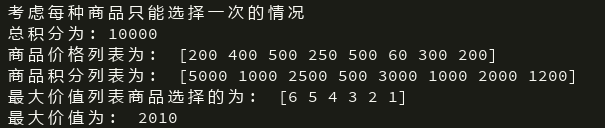
\includegraphics[scale=0.6]{../images/xiaomei_max_value.png}
	\caption{最大价值问题实验输入输出}
\end{figure}


\newpage
\section{分支限界与回溯}
\subsection{n个处理机和k个任务问题}
\subsubsection{问题描述}
假设有n个任务由k个可并行工作的机器完成。完成任务i需要的时间为 。试设计一个算法找出完成这
n个任务的最佳调度,使得完成全部任务的时间最早。
例如,输入为
\begin{lstlisting}[language=C]
7 3
2 2 14 4 16 6 5 3
\end{lstlisting}
表示有7个任务,有3台可并行工作的机器。每个任务需要的完成时间在第二行。
输出文件示例
\begin{lstlisting}[language=C]
1
17
\end{lstlisting}
\subsubsection{解决问题所用的算法设计方法及基本思想}
此问题采用的方法是分支限界,先然一个处理机处理所以任务,然后从这个处理机中
分出一个任务分给其它的处理机,这样一次一次的分配,直到三个处理机中最大的为所有情况中
最小时,返回,并且在此过程中记录每一次每个处理机中的处理情况。
\subsubsection{采用的数据结构描述}
使用一个二维数组来保存每个处理机处理任务的信息。
\subsubsection{算法描述 }
   {\bfseries 处理机调度} \\
   \tab{\bfseries{算法 nkSchedeling (dep, lens, t, n, k, result) }} \\
	\tab// 找出价值最大的商品集合 \\
	\tab// 输入:dep, lens, t, n, k, result\\
	\tab// 输出:result 包含处理机调度的数组 \\
	\tab{\bfseries if} dep = n {\bfseries do} \\
	\tab\tab tmp $\leftarrow$ comp(lens) // 找到一次中的最大时间\\
	\tab\tab{\bfseries if} tmp $<$ bestSoFar \\
	\tab\tab\tab bestSoFar = tmp\\
	\tab\tab{\bfseries return}\\
	\tab{\bfseries for} $i \leftarrow 0$ {\bfseries to} $k$ {\bfseries do} \\
	\tab\tab lens[i] += t[dep]\\
	\tab\tab result[dep] = i\\
	\tab\tab{\bfseries if} $lens[i] < bestSoFar$ {\bfseries do} \\
	\tab\tab\tab nkSchedeling(dep+1, lens, t, n, k, result) \\
	\tab\tab lens[i] -= t[dep]\\
	\tab\tab delete(result[dep])\\
\subsubsection{算法的时间空间复杂度分析 }
时间复杂度 $\Theta(n) = n^k$,空间复杂度为 $n^2$
\subsubsection{算法实例}
输入:
\begin{lstlisting}[language=C]
处理机个数:n = 3
任务个数:k = 7
每个任务所花时间:t = {2, 14, 23, 11, 9, 3, 4, 16, 6, 5, 3}
\end{lstlisting}

输出:
\begin{figure}[H]
	\centering
	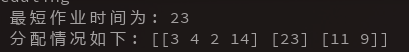
\includegraphics[scale=0.6]{../images/branch_and_output.png}
	\caption{处理机调度}
\end{figure}


\newpage
\section{附加题目}
\subsection{学习超市选址问题}
\subsubsection{问题描述}
学校超市选址问题 (带权有向图的中心点)
设计内容:对于某一学校超市,其他各单位到其的距离不同,同时各单位人员去超市的频度也不同。
请为超市选址,要求实现总体最优。
设计要求:
\begin{enumerate}
	\item 设计该问题的核心算法;
	\item 设计可视化的界面,界面中能有效显示学校超市可设立的地点和各单位的位置以及它们之间的有效路径;
	\item 程序能自动计算出最优设立点,并最好以图示化方式演示。
\end{enumerate}
\subsubsection{解决问题所用的算法设计方法及基本思想}
本题目采用Floyd最短路径算法,把每个点到其它点的距离全部算出来,然后
比较,选出距离最短的点。
\subsubsection{采用的数据结构描述}
使用二维矩阵来保存点与点之间的距离。
\subsubsection{算法描述 }
   {\bfseries 找出带权有向图的中心点} \\
   \tab{\bfseries{算法 findShortest (maxtrix) }} \\
	\tab// 找出带权有向图的中心点\\
	\tab// 输入:一个二维数组表示每个点之间的距离\\
	\tab// 输出:maxtrixS表示最终的点与点之间的最终距离\\
	\tab// 输出:pPath表示最终距离到最终距离的路径\\
	\tab maxtrixS $\leftarrow$ matrix\\
	\tab pPath $\leftarrow$ new array\\
	\tab{\bfseries for} $k \leftarrow 0$ to len(matrix) {\bfseries do} \\
	\tab\tab{\bfseries for} $i \leftarrow 0$ to len(matrix) {\bfseries do} \\
	\tab\tab\tab{\bfseries for} $j \leftarrow 0$ to len(matrix) {\bfseries do} \\
	\tab\tab\tab\tab min,po $\leftarrow$ min(maxtrixS[i,j],maxtrixS[i,k]+maxtrixS[k,j])\\
	\tab\tab\tab\tab maxtrixS[i,j] $\leftarrow$ minP\\
	\tab\tab\tab\tab append(path[i,j], k)\\
	\tab{\bfseries return} maxtrix, pPath\\
\subsubsection{算法的时间空间复杂度分析 }
本题的时间复杂度为 $\Theta(n) = n^3$,空间复杂度为 $n^3$。
\subsubsection{算法实例}
\begin{figure}[H]
	\centering
	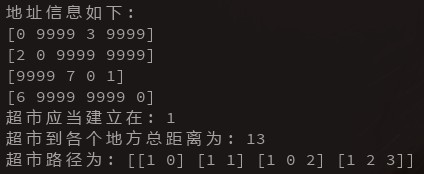
\includegraphics[scale=0.6]{../images/find_shortest_path.png}
	\caption{超市选址实例}
\end{figure}

\newpage
\section{课程设计总结}
本次的算法课程设计让我更加深刻的理解的一些基本的算法思想,包括蛮力法、分支限界、
回溯法、动态规划等。在每完成一道算法题时,都会对该算法思想具有更深刻的认识和体会,
即使有些比较困难,但最终都会得到很大的收获。

\end{document}
